\documentclass{article}

% Language setting
% Replace `english' with e.g. `spanish' to change the document language
\usepackage[english]{babel}

% Set page size and margins
% Replace `letterpaper' with `a4paper' for UK/EU standard size
\usepackage[letterpaper,top=2cm,bottom=2cm,left=3cm,right=3cm,marginparwidth=1.75cm]{geometry}

% Useful packages
\usepackage{amsmath}
\usepackage{graphicx}
\usepackage[colorlinks=true, allcolors=blue]{hyperref}

\title{CME211 Project Part 2 Pipe Wall Heat Distribution}
\author{Xuyi Long}

\begin{document}
\maketitle


\section{Project Summary}

For the final project we developed a C++ program to solve the 2D heat equations on a simple pipe wall geometry. The core of this program is the CG solver, which is an iterative algorithm that uses Conjugate Gradient method to solve for a linear system of equation Au = b, where A is a input matrix, u is the solution vector, b is a vector of zeros. The CG solver takes a CSR matrix, a initial guess of solution vector u0, and right hand side b, and a tolerance threshold value as input parameters. The program continues to execute until the solution value converged within the specified tolerance threshold[1]. The CG solver developed from part 1 was modified as part of Object Oriented Programming design[2], which consists of two classes: the SpareseMatrix class and the HeatEquation class.



\section{CG Solver Implementation}

This SparseMatrix class defines a sparse matrix object, which contains vectors defining the matrix as data attributes and methods to perform various tasks to take 2d array inputs and output a matrix in CSR format.

This HeatEquation2D class contains data attributes and method to form a system of equation from the input file. It takes a input file as an argument and instantiate matrix A as a SparseMatrix object and solve the system using the CG solver developed in part 1 of the project. The pseudocode for the CG algorithm is provided in page 2 of project part 1 handout [1]. 



\section{User Guide}
\begin{enumerate}
\item Compile the C++ program on the terminal. Run the makefile.

\item The main file with the input file and the prefix of the output solution. An example is provided below:

 \begin{verbatim}
$ ./main input1.txt solution
SUCCESS: CG Solver converged in 132 iterations.
\end{verbatim}

\begin{figure}[]
\centering
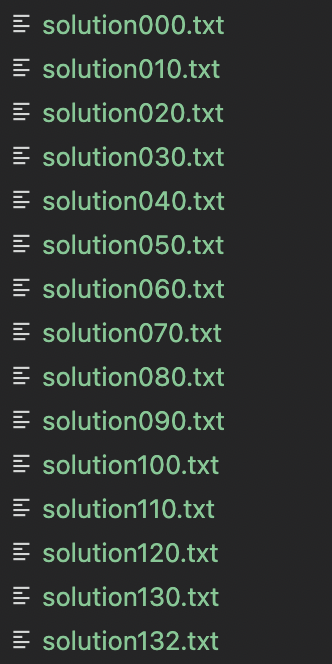
\includegraphics[width=0.3\textwidth]{solution_example.png}
\caption{\label{fig:frog}sample solution output for input1.txt}
\end{figure}

The output is a series of solution files that includes the last iteration. The output file should be generated every 10 iterations. Example output files are provided in figure 1.

\item To visualize the solution file, run the postprocess.py on the terminal using the input file and the desired solution file generated from the previous step. Here is an example of the python output.

 \begin{verbatim}
python3 postprocess.py input1.txt solution132.txt
Input file processed: input1.txt
Mean Temperature: 116.26631
\end{verbatim}


\end{enumerate}


\section{Example Figures}

The pseudo-color plots with mean temperature isolines generated from postprocess.py are shown in figure 2, 3, and 4. The x and y axis indicate the length and width of the pipe wall geometry. 

\begin{figure}[]
\centering
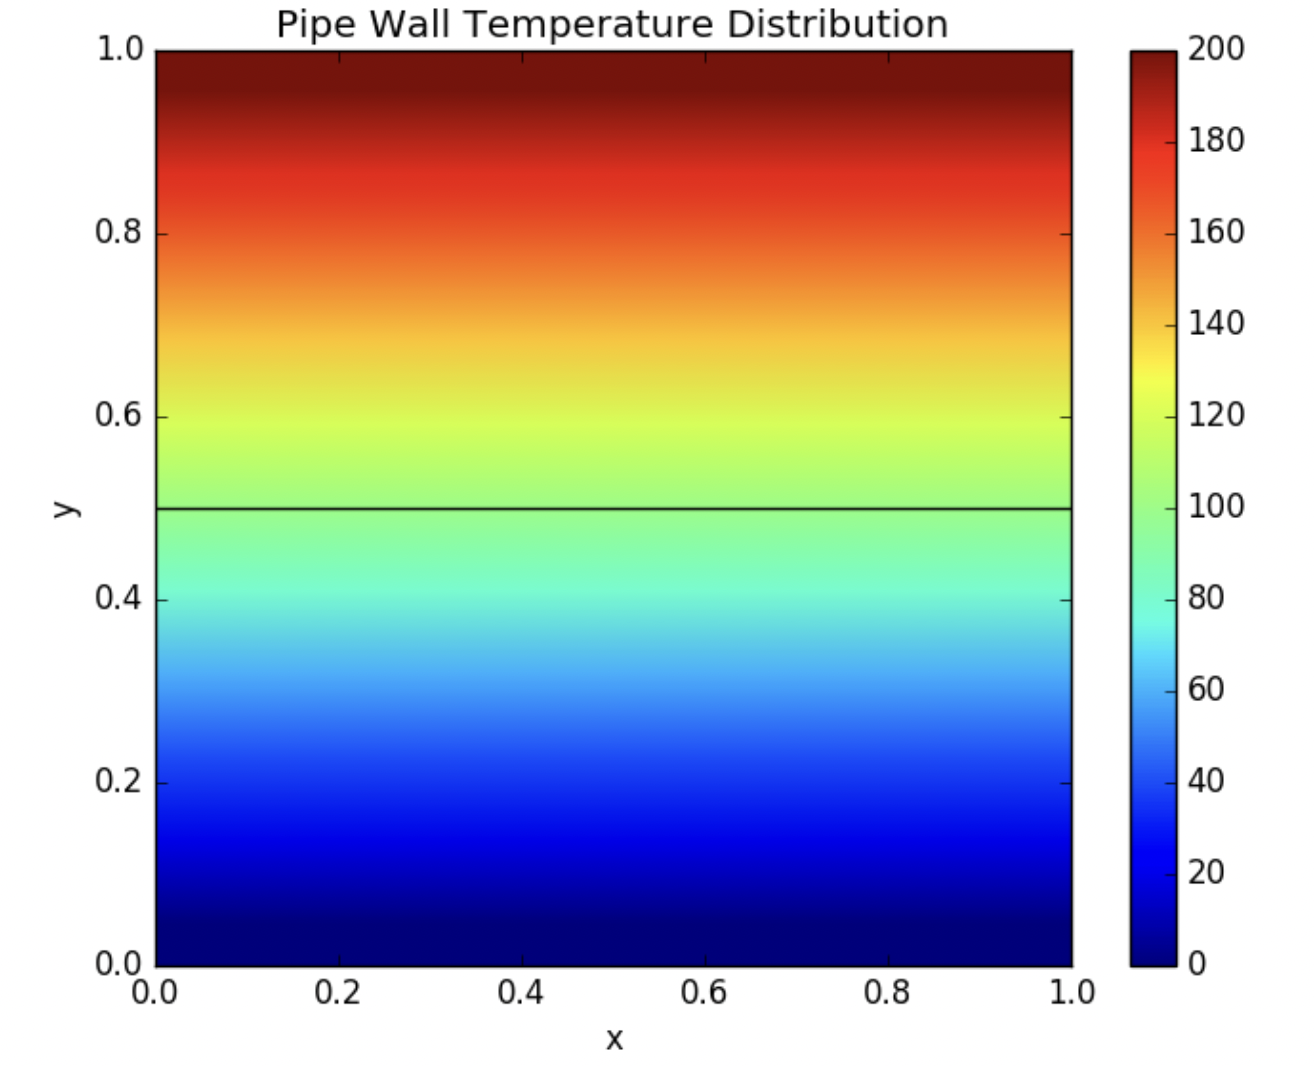
\includegraphics[width=0.6\textwidth]{input0plot.png}
\caption{\label{fig:frog}temperature distribution for input0.txt}
\end{figure}

\begin{figure}[]
\centering
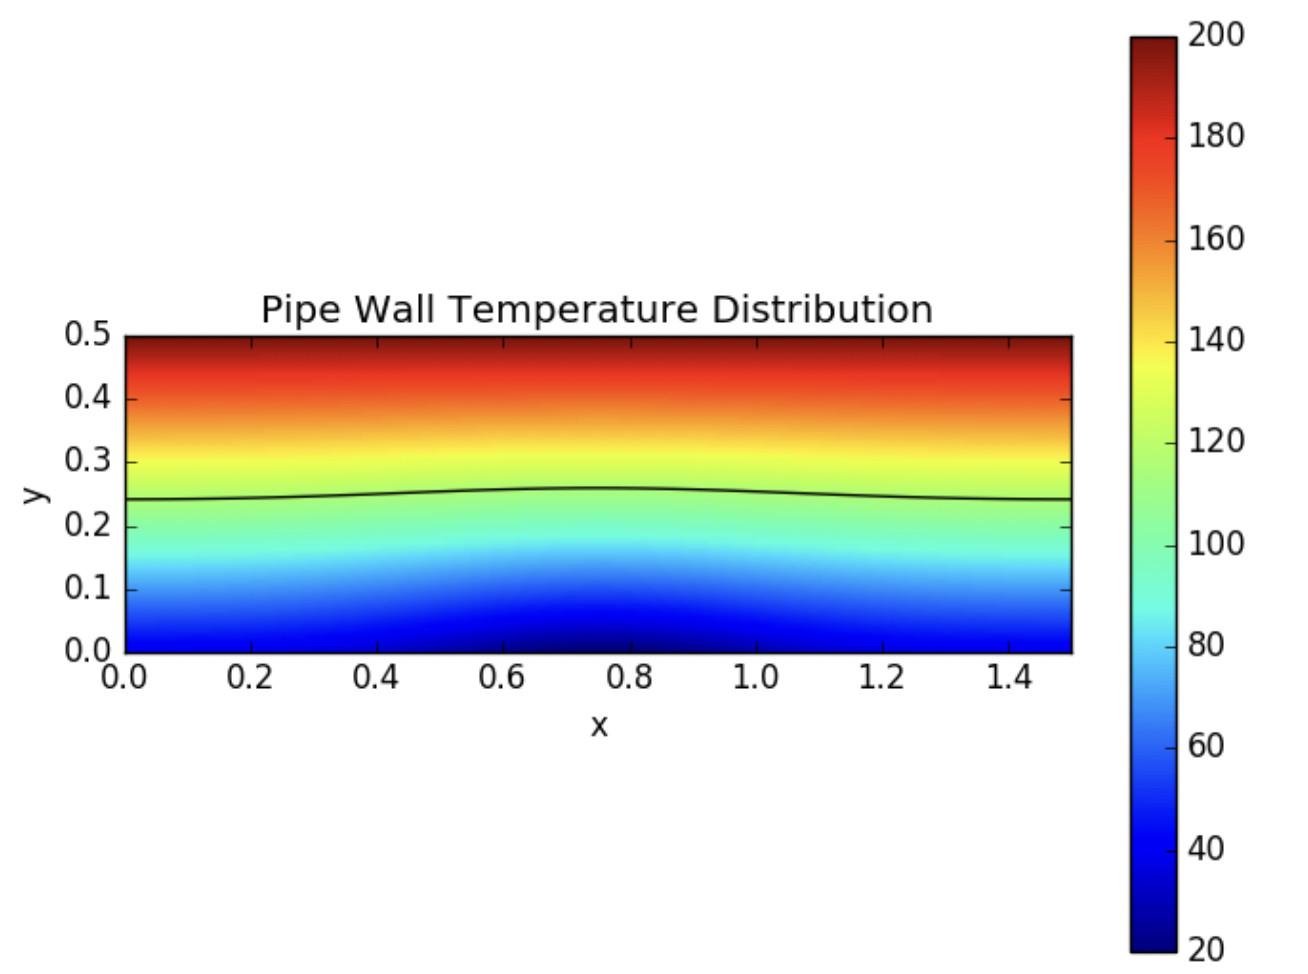
\includegraphics[width=0.6\textwidth]{input1plot.png}
\caption{\label{fig:frog}temperature distribution for input1.txt}
\end{figure}

\begin{figure}[]
\centering
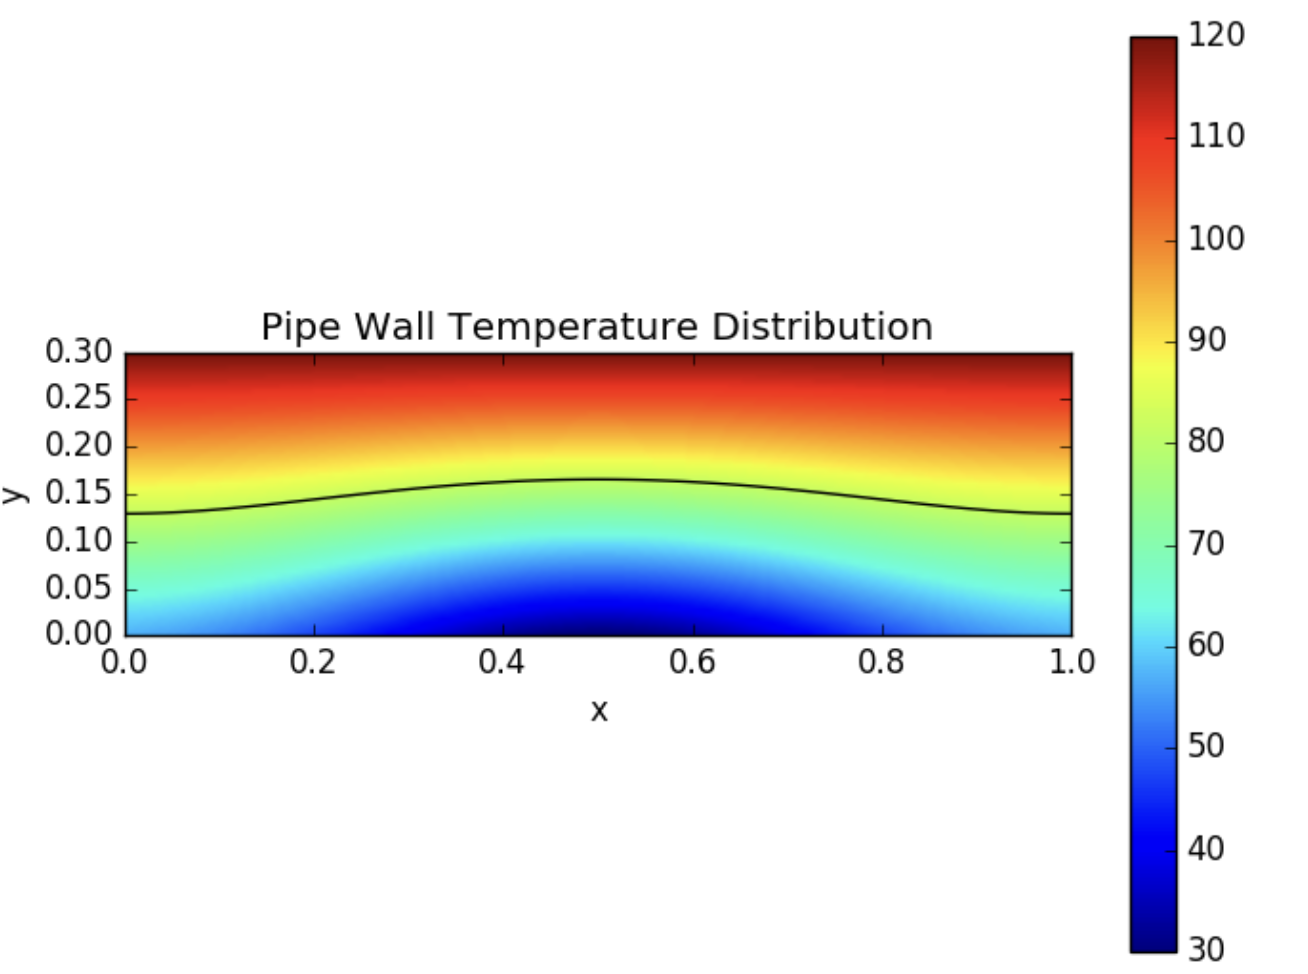
\includegraphics[width=0.6\textwidth]{input2plot.png}
\caption{\label{fig:frog}temperature distribution for input2.txt}
\end{figure}

\section{References}


\begin{enumerate}
\item CME 211 project part1 handout.
https://canvas.stanford.edu/courses/158790/files/folder
/Homeworks?preview=10598005

\item CME 211 project part2 handout. https://canvas.stanford.edu/courses/158790/files/folder
/Homeworks?preview=10685046

\end{enumerate}

\end{document}